\section{Coverage}
\sectionlabel{coverage}

To what extent does the scope graph framework cover name binding systems that live in the
world of real programming languages? It is not possible to \emph{prove} complete
coverage by the framework, in the sense of being able to encode all possible
name binding systems that exist or may be designed in the future.
(Indeed, given that these systems are typically implemented in compilers
with algorithms in Turing-complete programming languages, the framework is likely
\emph{not} to be complete.)
However, we believe that our approach handles many lexically-scoped languages.
The design of the framework was informed by an investigation of a wide range of
name binding patterns in existing languages, their (attempted) formalization in
the NaBL name binding language \cite{KatsV10,KonatKWV12}, and their encoding in scope
graphs.
In this section, we discuss three such examples: \pcfmcode{let} bindings, qualified names,
and inheritance in Java.
This should provide the reader with a good sense of how name binding patterns
can be expressed using scope graphs.
Appendix  \refcoverageappendix~of \cite{TUD-SERG-2015-001-local} provides further examples,
including definition-before-use, compilation units and packages in Java, and namespaces and partial classes in
C\#. 

\begin{figure}[t]
\begin{boxedminipage}{\hsize}
\centering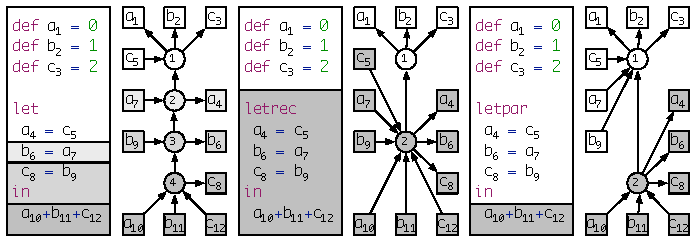
\includegraphics{figures/scope-graphs/lets/all.pdf}
\end{boxedminipage}
% \vspace{1ex}
% \hrule
\vspace*{-\baselineskip}
\caption{Example LM programs with sequential, recursive, and parallel \pcfmcode{let}, and
their encodings as scope graphs.}
\figurelabel{lm:lets}
\end{figure}

\paragraph{Let bindings.}

The several flavors of \pcfmcode{let} bindings in languages such as ML, Haskell, and
Scheme do not follow the unary lexical binding pattern in which the binding
construct dominates the abstract syntax tree that makes up its scope.
The LM language from \Figure{pcfm:grammar} has three flavors of \pcfmcode{let} bindings:
sequential, recursive, and parallel \pcfmcode{let}, each with a list of bindings and
a body expression.
\Figure{lm:lets} shows the encoding into scope graphs for each of the constructs
and makes precise how the bindings are interpreted in each flavour.
In the recursive \pcfmcode{letrec}, the bindings are visible in all initializing
expressions, so a single scope suffices for the whole construct.
In the sequential \pcfmcode{let}, each binding is visible in the
\emph{subsequent} bindings, but not in its own initializing expression. This
requires the introduction of a new scope for each binding.
In the parallel \pcfmcode{letpar}, the variables being bound are not
visible in any of the initializing expressions, but only in the body.
This is expressed by means of a single scope (2) in which the bindings are
declared; any references in the initializing expressions are associated to the
parent scope (1).

\begin{figure}[t]
\begin{minipage}[b]{0.49\textwidth}
\begin{boxedminipage}{\hsize}
\hspace*{-0.3cm}
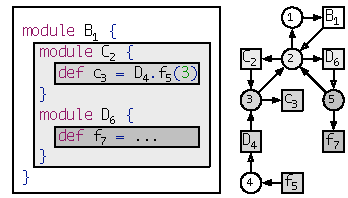
\includegraphics{figures/scope-graphs/qualified/example3.pdf}
\end{boxedminipage}
\caption{Example LM program with partially-qualified name.}
\figurelabel{lm:qualified}
\end{minipage}
\begin{minipage}[b]{0.49\textwidth}
\begin{boxedminipage}{\hsize}
\hspace*{-1.5mm}
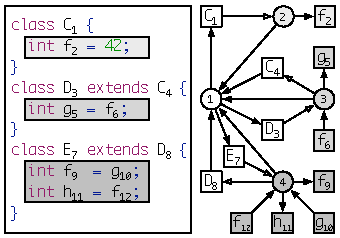
\includegraphics{figures/scope-graphs/inheritance/inheritance.pdf}
\end{boxedminipage}
\caption{Class inheritance in Java modeled by import edges.}
\figurelabel{java:inh}
\end{minipage}
\end{figure}



% \begin{wrapfigure}[11]{r}{0.51\textwidth}
% \vspace*{-2\baselineskip}
% \begin{boxedminipage}{\hsize}
% \centering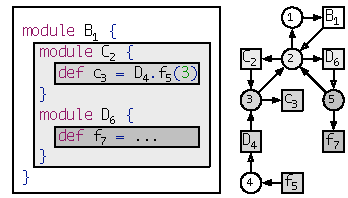
\includegraphics{figures/scope-graphs/qualified/example3.pdf}
% \end{boxedminipage}
% \caption{Example LM program with partially-qualfied name.}
% \figurelabel{lm:qualified}
% \end{wrapfigure}

\paragraph{Qualified names.}

Qualified names refer to declarations in named scopes outside the lexical scoping.
They can be either used as simple references or as imports.
For example, fully-qualified names of Java classes can be used to refer to (or import) classes
  from other packages.
While fully-qualified names allow navigating named scopes from the root scope,
partially-qualified names give access to lexical subscopes, 
  which are otherwise hidden from lexical parent scopes.

The LM program in \Figure{lm:qualified} uses a
partially-qualified name \pcfmcode{D.f} to access function \pcfmcode{f} in submodule \pcfmcode{D}.
We can model this pattern using an anonymous scope (4),
which is not linked to the lexical context. The relative name
(\pcfmcode{f}$_5$) is a reference in the anonymous scope.
We add the qualifying scope name (\pcfmcode{D}$_4$) as an import in the
anonymous scope. 
  
%\TODO{The declaration of a subpackage is never in scope.}

%\TODO{aliases: should probably be postponed to future work}

% \begin{wrapfigure}[14]{r}{0.51\textwidth}
% \vspace*{-1\baselineskip}
% \begin{boxedminipage}{\hsize}
% \centering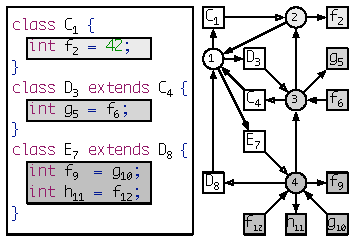
\includegraphics{figures/scope-graphs/inheritance/transitive.pdf}
% \end{boxedminipage}
% \caption{Class inheritance in Java modeled by import edges.}
% \figurelabel{java:inh}
% \end{wrapfigure}

\paragraph{Inheritance in Java.}

%As we alluded to in \Section{imports}, the concepts of named scopes and imports
%in the scope graph framework can be used to model more than just language
%constructs called `module'.
We can model
inheritance in object-oriented languages 
with named scopes and imports.
For example, \Figure{java:inh} shows a hierarchy of three Java classes.
Class \javacode{C} declares a field \javacode{f}.
Class \javacode{D} extends \javacode{C} and inherits its field \javacode{f}.   
Class \javacode{E} extends \javacode{D}, inheriting the fields of \javacode{C} and \javacode{D}.
Each class name is a declaration in the same package scope (1),
  and associated with the scope of its class body.
Inheritance is modeled with imports: a subclass body scope contains an import referring to its super class, making the declarations in the super class reachable from the body. In the example, the scope (4) representing the body of class \javacode{E} contains an import referring to its super class \javacode{D}. Using this import, \javacode{g}$_{10}$ correctly resolves to \javacode{g}$_{5}$ . Since local declarations hide imported declarations, \javacode{f}$_{12}$ also refers correctly to the local declaration \javacode{f}$_{9}$, which hides the transitively imported \javacode{f}$_{2}$.
Note that since a scope can contain several imports, encoding multiple inheritance uses exactly the same principle.
